\newpage
\section{常见的矩阵关系}
\begin{figure}[!htb]
    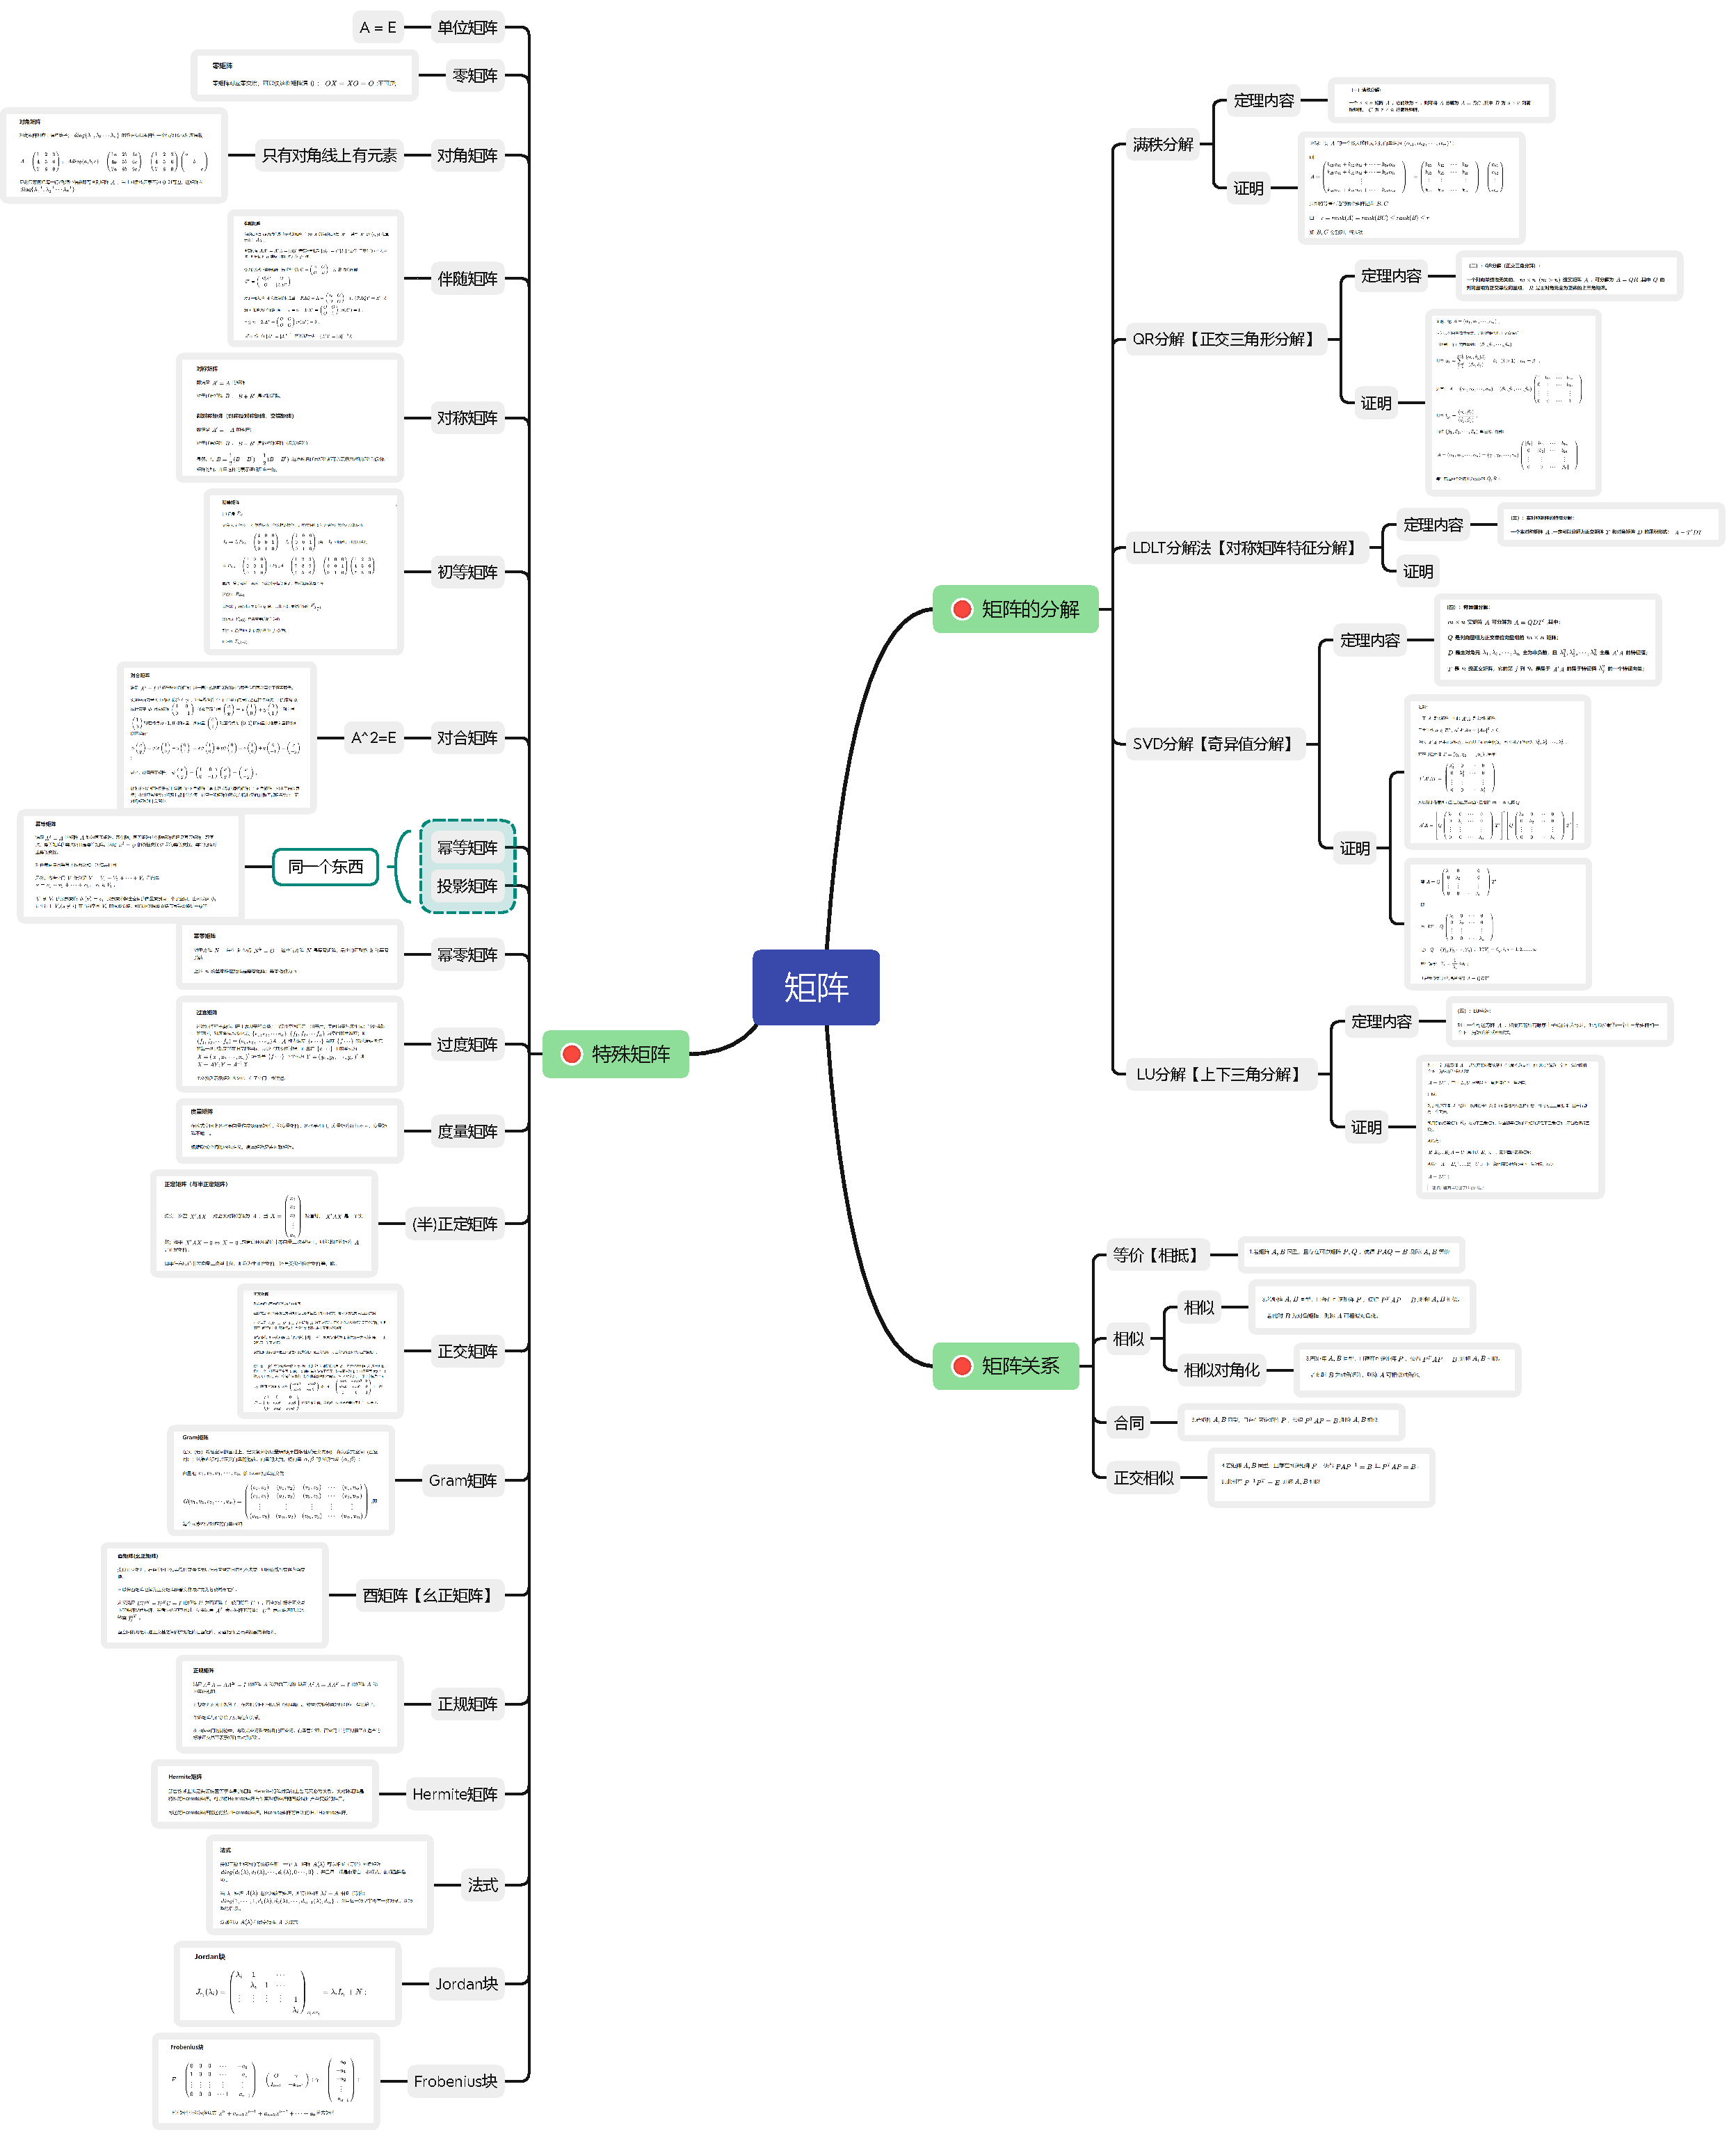
\includegraphics[scale=0.4]{Chapter/TikZ/矩阵.pdf}
    \label{矩阵}
    \caption{矩阵关系}
\end{figure}


\section{和式}
引入:看到一个双重求和的和式,但是我自己不会计算,很烦……
\begin{align*}
    \sum _{i=0}^n \left[\sum _{j=1}^{n-i} j^2\right]=\frac{1}{12} n (n+1)^2 (n+2)
\end{align*}

\textsf{轮换求和与对称求和}

两种形式
\[\sum_{cyc}^{}{}\hspace*{0.5\linewidth}\sum_{ sym}^{}{}\]

弄明白,尽量联系不等式里边的这两个东西。因为似乎在用了这个东西可以简化运算。

\subsection{轮换式中的根}
假如原来有一个根 $x =a$, 也就是说我们有$(x-a)(\cdots)= 0$。 
我们把$x\to y$, 可以得到$(y-a) (\cdots )=0$。 明显这个式子有一个根$y =a$。 
又因为这个式子是轮换的,所以可以得出后边的式子和前边的式子完全相同。
也就是说前边的式子一定有一个根$y =a$。 于是我们就可以知道原来的式子有两个根,
分别为$x = a, y=a$

\section*{求和符号基础知识}
\textsf{对称式:}三元任意换仍未原式

$x\Rightarrow y, y\Rightarrow z, z\Rightarrow x$.换完以后整体式子和原来恒等,比如$x+y+z, x^2 + y^2 + z^2, xy + yz + xz$ 

\textsf{对称式:}依序(正反序)互换后仍为原式
\newpage

\subsection{常见的和式恒等变换}
\begin{theorem}[和式恒等变换]
    \begin{align*}
    \num{1}\qquad & \left[\sum_{i=1}^{n}{a_i}\right]^2
        & = &\qquad\qquad \sum_{i=1}^{n}{a_i^2} + 2\sum_{1 \le i \le i \le n}{a_i a_j}\\
    % 
    % 
    \num{2}\qquad & \left[\sum_{1 \le i \le i \le n}{(a_i - a_j)}\right]^2
        & = &\qquad\qquad n\sum_{i=1}^{n}{a_i^2} - \left[\sum_{i=1}^{n}{a_i}\right]^2\\
    % 
    % 
    \num{3}\qquad & \left[\sum_{i=1}^{n}{a_i}\right] \left[\sum_{i=1}^{n}{b_i}\right]
        & = &\qquad\qquad \sum_{i=1}^{n}{\sum_{j=1}^{n}{a_i b_j}} = \sum_{j=1}^{n}{\sum_{i=1}^{n}{a_i b_j}}\\
    % 
    % 
    \num{4}\qquad & \left[\sum_{1 \le i \le i \le n}{a_ia_j}\right]^2
        & = &\qquad\qquad \sum_{i=1}^{n}{\sum_{j=1}^{n}{a_i a_j}} = \sum_{j=1}^{n}{\sum_{i=1}^{n}{a_i b_j}}\\
    % 
    %
    \num{5}\qquad & \sum_{i=1}^{n}{\sum_{j=1}^{n}{a_i a_j}}
        & = &\qquad\qquad \sum_{i=1}^{n}{a_i^2} + \frac{1}{2} \sum_{i=1}^{n}{\sum_{j=1}^{n}{[a_i b_j + a_j b_i]}}\\
    % 
    %
    \num{6}\qquad & \sum_{i=1}^{n-1}{\biggl(a_{i+1}-a_i\biggr)}
        & = &\qquad\qquad a_n-a_1\\
    % 
    %
    \num{7}\qquad & \sum_{i=1}^{n}{a_ib_i}
        & = &\qquad\qquad \sum_{i=1}^{n-1}{\bigg[(a_i-a_{i+1})B_i\bigg]} + a_nB_n\\
    % 
    %
    \num{8}\qquad & \sum_{i=m}^{n}{a_ib_i}
        & = &\qquad\qquad \sum_{i=m}^{n-1}{[(a_i-a_{i+1})B_i]} + a_nB_n - a_mB_{m-1}\\
    % 
    %
    \num{9}\qquad & \left[\sum_{i=1}^{n}{a_i^2}\right]\cdot \left[\sum_{i=1}^{n}{b_i^2}\right]
        & = &\qquad\qquad \left[\sum_{i=1}^{n}{a_ib_i}\right]^2 + \sum_{1\le i \le j \le n}({a_ib_j-a_jb_i})^2
    \end{align*}
\end{theorem}

\subsection{预备准备}
在证明之前,首先说明一个式子的几何意义,这对下面的证明有帮助
$\sum\limits_{1 \leq i<j \leq n} a_{i} a_{j} $,它的几何意义如下图,
其实就是一个 $(n-1)\times (n-1)$的上三角矩阵。

\begin{align*}
    \sum\limits_{1 \leq i<j \leq n} a_{i j}=
    \left|\begin{array}{cccc}
    a_{1} a_{2} & +a_{1} a_{3} & & +a_{1} a_{n} \\
    +a_{2} a_{3} & \cdots & +a_{2} a_{n} & \\
    \vdots & \ldots & & \\
    +a_{n-1} a_{n} & & & \\
    \end{array}\right|
\end{align*}


此外我们在这里引入另外一个记号$A$,具体的形式如下:
那么$A$旋转即可得到上边的$\sum\limits_{1 \leq i<j \leq n} a_{i j}$,其实$\sum\limits_{1 \leq i<j \leq n} a_{i j}$就是A的左下部分的旋转。

\begin{align*}
    {A}=\left|\begin{array}{ccccc}
    a_{1} a_{1} & & & \cdots & \\
    a_{2} a_{1} & a_{2} a_{2} & \cdots & & \\
    \cdots & \cdots & a_{3} a_{3} & & \\
    a_{n-1} a_{1} & \cdots & \cdots & \cdots & \\
    a_{n} a_{1} & a_{n} a_{2} & \cdots & a_{n} a_{n-1} & a_{n} a_{n}
    \end{array}\right|
\end{align*}



\subsection{等式的证明}
\begin{proof}\num{1}
    
\begin{align*}
    \left(\sum\limits_{i=1}^{n} a_{i}\right)^{2}
    & = \left(a_{1}+a_{2}+\cdots+a_{n-1}+a_{n}\right)^{2} \\
    & = a_{1}\left(a_{1}+a_{2}+\cdots+a_{n-1}+a_{n}\right)
    + a_{2}\left(a_{1}+a_{2}+\cdots+a_{n-1}+a_{n}\right) \\
    & \hspace*{16em}+ \cdots+a_{n}\left(a_{1}+a_{2}+\cdots+a_{n-1}+a_{n}\right) \\
    & = \left|
    \begin{array}{ccccc}
        a_{1} a_{1} & +a_{1} a_{2} & +a_{1} a_{3} & \cdots & +a_{1} a_{n} \\
        +a_{2} a_{1} & +a_{2} a_{2} & \cdots & & \\
        \cdots & \cdots & +a_{3} a_{3} & & \\
        +a_{n-1} a_{1} & \cdots & \cdots & \cdots & \\
        +a_{n} a_{1} & +a_{n} a_{2} & \cdots & +a_{n} a_{n-1} & +a_{n} a_{n}
    \end{array}
    \right|
     = \sum\limits_{\mathrm{i}=1}^{\mathrm{n}} a_{\mathrm{i}}^{2} + 2\sum\limits_{1 \leq i<j \leq n} a_{i} a_{j}\nonumber\\
    &\Longrightarrow \text{注:第i行即第i项}\nonumber
\end{align*}
\end{proof}


\begin{proof}\num{2}
\begin{align*}
    \sum_{1 \leq i<j \leq n}^{n}\left(a_{i}-a_{j}\right)^{2}
    & = \sum_{1 \leq i<j \leq n}^{n}\left(a_{i}^{2}-2 a_{i} a_{j}+a_{j}^{2}\right)\nonumber\\
    & = \left[\left(a_{1}^{2}-2 a_{1} a_{2}+a_{2}^{2}\right)+\cdots+\left(a_{1}^{2}-2 a_{1} a_{n}+a_{n}^{2}\right)\right] \\
    & + \left[\left(a_{2}{ }^{2}-2 a_{2} a_{3}+a_{3}^{2}\right)+\cdots+\left(a_{2}{ }^{2}-2 a_{2} a_{n}+a_{n}{ }^{2}\right)\right] 
      \quad + \left[\left(a_{n-1}^{2}-2 a_{n-1} a_{n}+a_{n}^{2}\right)\right]\\
    & = (n-1) \sum\limits_{i=1}^{n} a_{i}{ }^{2}-2\cdot
    \left|
    \begin{array}{cccc}
        a_{1} a_{2} & +a_{1} a_{3} & & +a_{1} a_{n} \\
        +a_{2} a_{3} & \cdots & +a_{2} a_{n} & \\
        \vdots & \ldots & & \\
        +a_{n-1} a_{n} & & & \\
    \end{array}
    \right|\\
    & =(n-1) \sum_{i=1}^{n} a_{i}{ }^{2}-2 \sum_{1 \leq i<j \leq n}^{n} a_{i} a_{j}\\
    & = n \sum_{i=1}^{n} a_{i}{ }^{2}-\left(\sum_{i=1}^{n} a_{i}{ }^{2}+2 \sum\limits_{1 \leq i<j \leq n}^{n} a_{i} a_{j}\right)
      = n \sum\limits_{i=1}^{n} a_{i}^{2}-\sum_{i=1}^{n} a_{i}^{2}
\end{align*}
\end{proof}


\begin{proof}\num{3}

\begin{align*}
    \left[\sum_{i=1}^{n} a_{i}\right]\times\left[\sum_{j=1}^{n} b_{j}\right]
    &=\left|
    \begin{array}{ccccc}
        a_{1} b_{1} & +a_{1} b_{2} & +a_{1} b_{3} & \cdots & +a_{1} b_{n} \\
        +a_{2} b_{1} & +a_{2} b_{2} & \cdots & \\
        \cdots & \cdots & +a_{3} b_{3} & & \\
        +a_{n-1} b_{1} & \ldots & \cdots & \cdots & \\
        +a_{n} b_{1} & +a_{n} b_{2} & \cdots & +a_{n} b_{n-1} & +a_{n} b_{n}
    \end{array}\right| \\
    &=a_{1} \sum_{j=1}^{n} b_{j}+a_{2} \sum_{j=1}^{n} b_{j}+\cdots+a_{n} \sum_{j=1}^{n} b_{j} \\
    &=\sum_{i=1}^{n}\left[a_{i}\left(\sum_{j=1}^{n} b_{j}\right)\right]
    =\sum_{i=1}^{n}\left[\left(\sum_{j=1}^{n} a_{i} b_{j}\right)\right] \\
    &=\sum_{i=1}^{n} \sum_{j=1}^{n} a_{i} b_{j}=\sum_{j=1}^{i \leftrightarrow j} \sum_{i=1}^{n} a_{j} b_{i} 
    =\sum_{j=1}^{n} \sum_{i=1}^{n} a_{i} b_{j}
    \Longrightarrow\text { 多重求和可以改变求和次序 }
\end{align*}
\end{proof}

\clearpage
\begin{proof}\num{4}

\begin{align*}
    \sum\limits_{1 \leq i<j \leq n} a_{i j}
    &=\left|
    \begin{array}{cccc}
        a_{1}a_{2} & +a_{1} a_{3} & & +a_{1} a_{n} \\
        +a_{2} a_{3} & \cdots & +a_{2} a_{n} & \\
        \vdots & \ldots & & \\
        +a_{n-1} a_{n} & & &\\
    \end{array}
    \right|\\
    &=a_{1}\sum_{j=1+1}^{n} a_{j}+a_{2} \sum_{j=2+1}^{n} a_{j}+\cdots+a_{n-1} \sum_{j=(n-1)+1}^{n} a_{j}
    \Longrightarrow\mbox{以前标为基准, i为前标} \\
    &=\sum_{i=1}^{n-1}\left[a_{i}\left(\sum_{j=i+1}^{n} a_{j}\right)\right] 
    =\sum_{i=1}^{n-1}\left[\sum_{j=i+1}^{n} a_{i} a_{j}\right]
    =\sum_{i=1}^{n-1} \sum_{j=i+1}^{n} a_{i} a_{j}\\
    & \Longrightarrow\mbox{以}45^{\circ}\mbox{线为轴:以斜标为基准, j为前标}\\
    & = \left(a_{1}\right) a_{2}+\left(a_{1}+a_{2}\right) a_{3}+\cdots+\left(a_{1}+a_{2}+\cdots+a_{n-1}\right) a_{n}\\
    & = a_{2} \sum_{j=1}^{2-1} a_{j}+a_{3} \sum_{j=1}^{3-1} a_{j}+\cdots+a_{n}\sum_{j=1}^{n-1} a_{j}\\
    & =\sum_{i=2}^{n}\left[a_{i}\left(\sum_{j=1}^{i-1} a_{j}\right)\right]
    =\sum_{i=2}^{n}\left[\left(\sum_{j=1}^{i-1} a_{i} a_{j}\right)\right] \\
    & =\sum_{i=2}^{n} \sum_{j=1}^{i-1} a_{i} a_{j} \Longrightarrow  \mbox{注:先取定外面的i值再展开内层}\\
\end{align*}

若以后标为基准将方阵变化一下即有:
\begin{align*}
 LHS&=\left|
    \begin{array}{ccccc}
        +a_{1} a_{2} & +a_{2} a_{3} & +a_{3} a_{4} & \cdots & a_{n-1} a_{n} \\
        +a_{1} a_{3} & +a_{2} a_{4} & \vdots & \cdots& \\
        +a_{1} a_{4} & \vdots & +a_{3} a_{n} & & \\
        \vdots & +a_{2} a_{n} & & & \\
        +a_{1} a_{n} & & &
    \end{array}
    \right|
\end{align*}
由对偶性知($i, j$只是一个记号而已), 
\[
    LHS=\sum_{j=1}^{n-1}\sum_{i=j+1}^{n}a_{i}a_{j}    
\]
\end{proof}



\begin{proof}\num{5}
\begin{align}
\sum_{i=1}^{n}{\sum_{j=1}^{n}{a_i a_j}}
&=\frac{1}{2}\left(\sum_{{i}=1}^{{n}} \sum_{{j}=1}^{{n}} a_{{i}} {b}_{{j}}+\sum_{{i}=1}^{{n}} \sum_{{j}=1}^{{n}} a_{{i}} {b}_{{j}}\right) \nonumber\\
&=\frac{1}{2} \sum_{{i}=1}^{{n}} \sum_{{j}=1}^{{n}}\biggl[a_{{i}} {b}_{{j}}+a_{{j}} {b}_{{i}}\biggr]\nonumber
\end{align}
\end{proof}

\begin{proof}\num{6}
\begin{align*}
    \sum_{i=1}^{n-1}\left(a_{i+1}-a_{i}\right)
    &=\left(a_{2}-a_{1}\right)+\left(a_{3}-a_{2}\right)+\ldots+\left(a_{n}-a_{n-1}\right) \\
    &=\left(a_{n}-a_{n-1}\right)+\ldots+\left(a_{3}-a_{2}\right)+\left(a_{2}-a_{1}\right) \\
    &=a_{n}-a_{1}
    \Longrightarrow\mbox{此式即为伸缩求和}
\end{align*}
\end{proof}
\clearpage


\begin{proof}\num{7, 8}

证法一

首先把所有的 $\mathrm{i}\rightarrow \mathrm{i}+1 $, 于是有 $n\to n-1$. 证法一(图解法),见陈纪修课本
\begin{align*}
    \sum_{i=2}^{n} A_{i-1} b_{i}=\sum_{i=1}^{n-1} A_{i} b_{i+1}
\end{align*}


证法二

\begin{align*}
    \sum_{i=m}^{n} a_{i} b_{i} 
    &=\sum_{i=m}^{n}\left[\left(A_{i}-A_{i-1}\right) b_{i}\right]
        = \sum_{i=m}^{n} A_{i} b_{i}-\sum_{i=m}^{n} A_{i-1} b_{i} \\
    &=\left(\sum_{i=m}^{n-1} A_{i} b_{i}+A_{n} b_{n}\right)-\sum_{i=m-1}^{n-1} A_{i} b_{i+1}
        \Longrightarrow\text { 把 } A_{i-1} \text { 变为 } A_{i} \text {, 方便后边提取公因式 } \\
    &=\sum_{i=m}^{n-1} A_{i} b_{i}+A_{n} b_{n}-\left[\sum_{i=m}^{n-1} A_{i} b_{i+1}+A_{\mathrm{m}-1} b_{m}\right]
        \Longrightarrow\text { 把求和范围变为相同 } \\
    & =\sum_{i=m}^{n-1}\left(A_{i} b_{i}-A_{i} b_{i+1}\right)+A_{n} b_{n}-A_{m-1} b_{m}
        =\sum_{i=m}^{n-1} A_{i}\left(b_{i}-b_{i+1}\right)+A_{n} b_{n}-A_{m-1} b_{m}\\
    &\mbox{注: 此式即为Abel分部求和}
\end{align*}

 
证法三

\begin{align*}
    \sum_{i=1}^n a_i b_i
    &=a_1 b_1+a_2 b_2+a_3 b_3+\cdots+a_n b_n \\
    &=b_1\left(A_1-A_0\right)+b_2\left(A_2-A_1\right)
        +b_3\left(A_3-A_2\right)+\cdots+b_n\left(A_{n-1}-A_n\right) \\
    &=\left(b_1-b_2\right) A_1+\left(b_2-b_3\right) A_2+\left(b_4-b_3\right) A_3
        +\cdots+\left(b_{n-1}-b_n\right) A_{n-1}+b_n A_n-b_1 A_0 \\
    &=\sum_{i=1}^{n-1} A_i\left(b_i-b_{i+1}\right)+b_n A_n
\end{align*}
\end{proof}


\begin{theorem}[Abel分部求和]
    \begin{align}
        \sum_{i=m}^{n}{a_ib_i}=\sum_{i=m}^{n-1} A_{i}\left(b_{i}-b_{i+1}\right)+A_{n} b_{n}-A_{m-1} b_{m}
    \end{align}
\end{theorem}

\textsf{关于Abel分部求和公式的几点讨论}

\ensuremath{\langle 1 \rangle} 若定义 $A_0=0$ ,那么当 $m=1$ 时即有
\[
    \sum_{i=1}^n a_i b_i 
    = \sum_{i=1}^{n-1} A_i\left(b_i-b_{i+1}\right)+A_n b_n
\]

\ensuremath{\langle 2 \rangle} 若 $a_i$ 不便于求和,那么便有如下的Abel和差变换
\[
    \sum_{i=m}^n\left(A_i-A_{i-1}\right) b_i 
    = \sum_{i=m}^{n-1} A_i\left(b_i-b_{i+1}\right)+A_n b_n-A_{\mathrm{m}-1} b_m
\]

\clearpage

\begin{proof}\num{9}
    \begin{align*}
    &\left(\sum_{i=1}^n a_i^2\right)\left(\sum_{i=1}^n b_i^2\right)-\sum_{i=1}^n\left(a_i b_i\right)^2
        = \sum_{i=1}^n \sum_{j=1}^n a_i^2 b_j^2-\sum_{i=1}^n \sum_{j=1}^n a_i b_i a_j b_j \\
    & = \frac{1}{2} \sum_{i=1}^n \sum_{j=1}^n\left(a_i{ }^2 b_j^2-2 a_i b_i a_j b_j+a_j{ }^2 b_i{ }^2\right)
        =\frac{1}{2} \sum_{i=1}^n \sum_{j=1}^n\left(a_i b_j-a_j b_i\right)^2 \\
    & = \sum_{1 \leq i<j \leq n}\left(a_i b_j-a_j b_i\right)^2
    \end{align*}
    注:柯西不等式即证毕
\end{proof}

\begin{theorem}[拉格朗日恒等式]
    \begin{align}
        \left[
        \sum_{i=1}^{n}{a_i^2}
        \right]
        \cdot 
        \left[
        \sum_{i=1}^{n}{b_i^2}
        \right]
        &=
        \left[
        \sum_{i=1}^{n}{a_ib_i}
        \right]^2
        +
        \sum_{1\le i \le j \le n}({a_ib_j-a_jb_i})^2
    \end{align}
\end{theorem} 